%%% tech_notes.tex --- Technical notes about multitask sfan.

\documentclass[12pt,a4paper]{article}
\usepackage[T1]{fontenc}     
\usepackage[utf8]{inputenc}            % Accents codés dans la fonte
% \usepackage[frenchb]{babel}            % Les traductions françaises

\usepackage[runin]{abstract}           % Section "Résumé"
\usepackage{amssymb}                   % Symboles mathématiques
\usepackage{amsmath}                   % Plus de symboles mathématiques
\usepackage{enumitem}                  % Personalisation des listes
\usepackage[margin=2cm]{geometry}      % Gestion des dimensions des pages
\usepackage{graphicx}                  % Gestion des inclusions graphiques
\usepackage{hyperref}                  % Inclusion d'URLs et de liens hypertexte
\usepackage[svgnames]{xcolor}          % Pour la gestion des couleurs

% Hyperref
% for a list of colors: p38 of http://mirrors.ibiblio.org/CTAN/macros/latex/contrib/xcolor/xcolor.pdf
\hypersetup{colorlinks=true,    % false: boxed links; true: colored links
            linkcolor=teal,     % color of internal links
            citecolor=teal}     % color of links to bibliography
% Font
\usepackage[bitstream-charter]{mathdesign}


% Mathematical notations
\newcommand{\sset}{\mathcal{S}}
\newcommand{\vset}{\mathcal{V}}
\DeclareMathOperator*{\argmax}{arg\,max}


\newcommand{\caz}[1]{{\color{purple}[TODO (CA) : #1]}}


\title{Multitask selection of features as nodes}
\author{Chloé-Agathe Azencott}
\date{March 2016}

\begin{document}

\maketitle


\section{Introduction}
% L'analyse de données génome entier dans le but de déterminer quelles régions du génome sont associées à un phénotype particulier sont souvent limitées par la faiblesse du nombre d'échantillons étudiés devant celui de variables mesurées. Ce phénomène statistique est particulièrement amplifié dans le cas des études type GWAS (Genome-Wide Association Studies), dans lesquelles les variables mesurées sont des mutations d'une paire de bases (Single Nucleotide Polymorphisms, ou SNPs) au nombre de plusieurs centaines de milliers. \\

% On parlera ainsi dans la suite de SNPs mais il pourrait tout aussi bien s'agir d'autres variables génomiques (expression de gène, méthylation, etc).\\

% Traditionnellement, ces études utilisent un test statistique pour évaluer l'association entre chaque SNP et le phénotype étudié, indépendamment les uns des autres. Elles ne prennent ainsi aucunement en compte la possibilité d'une interaction entre ces SNPs. Cependant, même un modèle linéaire (qui ne suppose donc que des effets additifs) souffre de ce problème de grande dimensionalité. En effet, une régression linéaire cherchant à expliquer le phénotype $y$ comme une combinaison linéaire $\sum_{j=1}^p w_j x_j$ des $p$ SNPs résultera en un système sous-déterminé : il n'y a pas de solution unique pour les poids $\{w_j\}_{j=1, \dots, p}$. \\

% Afin de restreindre le nombre de solutions possible, il est fréquent dans ce cas d'imposer des contraintes sur l'espace des solutions. On parle alors de régularisation. C'est par exemple ce que fait l'approche du Lasso (Least absolute shrinkage and selection operator)~\cite{tibshirani96}, qui impose de mettre un grand nombre de coefficients à zéro. On parle alors de {\it parcimonie} (ou \og sparsité \fg, de l'anglais {\it sparsity}). Le Lasso est une méthode de {\it sélection de variables} ({\it feature selection} en anglais), au sens où seules les variables ayant un coefficient non-nul sont sélectionnées pour être utilisées dans le modèle final.

\section{Related Work}
\subsection{SConES}
% Plus récemment, des travaux ont émergé pour imposer des contraintes supplémentaires, et en particulier pour forcer les variables sélectionnées à respecter une structure de réseau pré-définie. En particulier, nous avons proposé en 2013 une approche appelée SConES (Selecting Connected Explanatory SNPs)~\cite{azencott13} qui permette de sélectionner des SNPs qui soient (1) associés au phénotype ; (2) peu nombreux ; (3) connectés sur un réseau biologique donné. 

\paragraph{Formulation}
% Étant donnés
% \begin{itemize}
% \item $\vset$ un ensemble de variables / SNPs de taille $p$ ($\vset = \{1, \dots, p\}$) ;  
% \item $\lambda, \eta \in \mathbb{R}^+$ deux hyperparam\`etres ;
% \item un réseau de $p$ nœuds, correspondant aux $p$ SNPs, représenté par sa matrice d'adjacence $W$ ;
% \item $X \in \{0, 1, 2\}^{n \times p}$ le génotype de ces $p$ SNPs pour $n$ échantillons (chaque SNP est représenté par le nombre d'allèles mineurs) ;
% \item $y \in \mathbb{R}^n$ le phénotype de ces $n$ échantillons,
% \end{itemize}

% on commence par calculer l'importance  $c_1, \dots, c_p$ des $p$ SNPs pour le phénotype donné. On utilise pour cela un test statistique, Linear SKAT~\cite{wu11}, qui suppose un modèle additif sur les SNPs. On peut aussi utiliser, par exemple, la corrélation de Pearson entre $X$ et $y$.\\

% On cherche ensuite à trouver le sous-ensembles $\sset$ de $\vset$ tel que : 
\begin{equation}
\argmax_{\sset \subseteq \vset }  \sum_{i \in \sset} c_i - \eta |\sset|
- \lambda \sum_{i \in \sset} \sum_{j \notin \sset} W_{ij} 
\label{eq:scones}
\end{equation}

% $\sset$ maximise la somme de trois termes :
% \begin{enumerate}
% \item $\sum_{i \in \sset} c_i$ est l'importance de $\sset$ pour le phénotype ;
% \item $- \eta |\sset|$ est d'autant plus grand que le nombre de variables sélectionnées ($|\sset|$) 
%       est faible : ce terme encourage la parcimonie ;
% \item $- \lambda \sum_{i \in \sset} \sum_{j \notin \sset} W_{ij} $ est d'autant plus petit qu'il existe de liens
%       dans le réseau connectant une variable sélectionnée à une variable non sélectionnée : 
%       ce terme encourage la sélection de variables connectées sur le réseau.
% \end{enumerate}

% Les paramètres $\lambda$ et $\eta$ contrôlent l'importance accordée aux termes de régularisation.

\paragraph{Solution}
% Cette formulation présente l'avantage d'être équivalente à un problème de coupe minimale $s/t$ sur un réseau que l'on peut construire à partir des données et présenté sur la Figure~\ref{fig:mincut_scones}. Le problème des coupes minimales est bien connu et il existe de nombreux algorithmes de flux maximal (mincut/maxflow) pour le résoudre.


\begin{figure}[h]
  \centering
  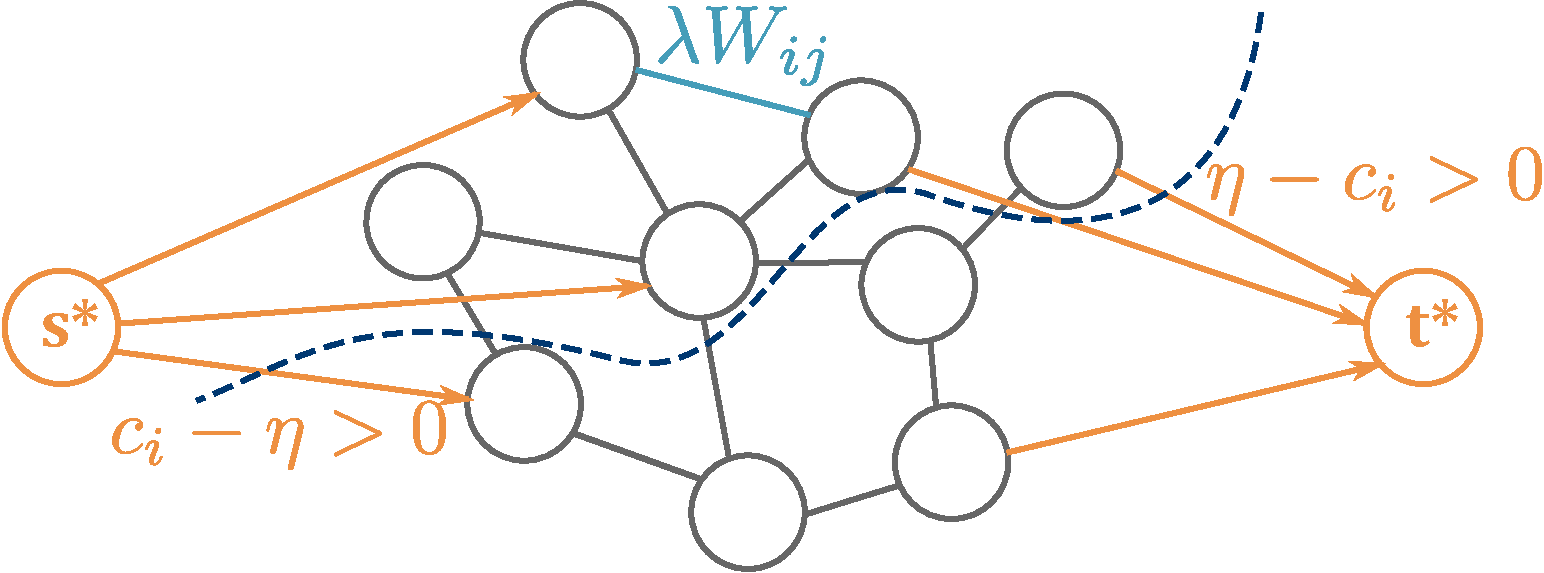
\includegraphics[width=0.7\textwidth]{figures/mincut_scones}
  \caption{Finding the minimum cut of this network is equivalent to solving the SConES optimization problem defined by ~\ref{eq:scones}.}
  \label{fig:mincut_scones}
\end{figure}


\subsection{MultiSConES}
% Une autre façon de réduire l'écart entre le nombre de variables et le nombre d'échantillons est d'augmenter le nombre d'échantillons. Cela peut être fait \og virtuellement \fg~si l'on dispose d'échantillons (les mêmes ou d'autres) pour lesquels d'autres phénotypes proches de celui qui nous intéresse ont été mesurés. Dans ce cas, on cherche à résoudre tous les problèmes de sélection de variable (correspondant à chaque phénotype) simultanément. C'est ce qu'on appelle une approche multi-tâches.\\

% Nous avons proposé en 2014 une extension multi-tâches de SConES, MultiSConES~\cite{sugiyama14}. Dans ce travail, on maximise une fonction qui comporte deux termes : 
% \begin{enumerate}
% \item La somme, pour les $K$ tâches, de la fonction optimisée pour SConES (Eq.~\ref{eq:scones}) ;
% \item Un terme $\mu \sum_{k=2}^K |\sset_{k-1} ~\Delta~ \sset_{k}| $ qui contrôle la différence symmétrique entre les ensembles de variables sélectionnées pour les différentes tâches.
% \end{enumerate}

% Cette nouvelle formulation peut aussi se résoudre par une reformulation mincut/maxflow.

\begin{equation}
\argmax_{\sset_1, \dots, \sset_K \subseteq \vset }  \sum_{k=1}^K \left (
\sum_{i \in \sset_k} c_i^k - \eta |\sset_k| - 
\lambda \sum_{i \in \sset_k} \sum_{j \notin \sset_k} W_{ij}^k \right ) - 
\mu  \sum_{k=1}^K \sum_{l > k} |\sset_{k} ~\Delta~ \sset_{l}|
\label{eq:multi_scones}
\end{equation}


\subsection{Using a matrix of task covariance}
% L'approche MultiSConES ne permet pas de prendre en compte la similarité entre les tâches : on ne peut pas encourager les tâches les plus similaires à partager le plus de variables. Par exemple, nous avions étudié des génotypes liés à la croissance des plantes ; bien que ces phénotypes aient vraisemblablement un certain nombre de facteurs communs, on peut imaginer que les facteurs déterminant la hauteur de la plante après 4 semaines de croissance (phénotype 1) aient plus en commun avec ceux déterminant la  hauteur de la plante après 8 semaines de croissance (phénotype 2) qu'avec ceux déterminant le nombre de feuilles de la plante (phénotype 3).\\

\paragraph{Formulation}
% Nous proposons donc ici une nouvelle formulation, dans laquelle le terme\\ $\sum_{k=2}^K |\sset_{k-1} ~\Delta~ \sset_{k}|$ est remplacé par un terme qui prenne en compte une matrice de similarités (ou corrélations) entre les tâches. Nous formulons donc le problème ci-dessous.

% Étant donnés
% \begin{itemize}
% \item $\vset$ un ensemble de $p$ variables ;
% \item $\lambda, \mu, \eta \in \mathbb{R}^+$ trois param\`etres ;
% \item $K$ réseaux, représentés par leurs matrices d'adjacence $W^1, \dots, W^K$, dont les nœuds appartiennent à $\vset$ ;
% \item $K$ vecteurs $c_1^k, \dots, c_p^k$ pondérant chacun les nœuds du réseau $W^k$ ($c_i^k$ représente l'importance de la variable $i$ pour la tâche $k$);
% \item une matrice $\Omega$ de taille $K \times K$ de corrélations entre tâches,  
% \end{itemize}

% on cherche à trouver les sous-ensembles $\sset_1, \dots, \sset_K$ de $\vset$ tels que : 

\begin{equation}
\argmax_{\sset_1, \dots, \sset_K \subseteq \vset } \sum_{k=1}^K \left ( \sum_{i \in \sset_k} (c_i^k - \eta)
- \lambda \sum_{i \in \sset_k} \sum_{j \notin \sset_k} W_{ij}^k \right )
- \mu \sum_{k=1}^K \sum_{l=1}^K \sum_{i \in \sset_k \setminus \sset_l} \Omega_{kl}^{-1}
\label{eq:msfan}
\end{equation}

% $\sum_{k=1}^K \sum_{l=1}^K \sum_{i \in \sset_k \cap \sset_l} \Omega_{kl}^{-1}$ est un terme d'autant plus petit que l'on a sélectionné les mêmes nœuds pour des tâches corrélées.\\

% $\lambda$, $\eta$ et $\mu$ permettent de moduler le r\^ole de chaque terme.\\

% Cette formulation recouvre les deux formulations précédentes :
% \begin{itemize}
% \item Si $\mu=0$, alors le problème est équivalent à SConES (Eq.~\ref{eq:scones}) pour chaque tâche indépendamment.
% \item Si $\Omega$ est définie par 
%   \[
%   \Omega_{kl} = 
%   \begin{cases}
%      \frac{1+\epsilon}{\epsilon (K + \epsilon)} & \mbox{ if } $k=l$ \\
%      \frac{1}{\epsilon (K + \epsilon)} & \mbox{otherwise},
%   \end{cases}
%   \]
%   avec $\epsilon > 0$, alors le problème est équivalent à MultiSConES (sans matrice de corrélation). 
% \end{itemize}

\paragraph{Solution}
% Cette formulation est équivalente à trouver une coupe minimale sur le super-réseau défini en connectant entre eux les $K$ réseaux ($W^1, \dots, W^K$) comme suit. \\

% On définit un nœud par couple (variable, tâche). 
% \begin{itemize}
% \item Un nœud $(i, k)$ est connecté au nœud $(i, l)$ (même variable, tâche différente) 
%     par une arête de poids $\mu \Omega_{kl}^{-1}$. 
% \item Un nœud $(i, k)$ est connecté au nœud $(j, k)$  (même tâche, variable différente) 
%     par une arête de poids $\lambda W_{ij}^{k}$. 
% \end{itemize}

% Pour chaque tâche on définit $\phi_k = \sum_{l=1}^K \Omega_{kl}^{-1}$.
% On ajoute au super-réseau deux nouveaux nœuds, une source $s*$ et un puits $t*$, 
% que l'on relie à chaque nœud $(i, k)$ de la façon suivante :
% \begin{itemize}
% \item Si $a_i^k = c_i^k - \mu \phi_k - \eta \geq 0$, alors on crée un arc (orienté) 
%     depuis $s*$ vers $(i, k)$, pondéré par $a_i^k$.
% \item Sinon, on crée un arc (orienté) depuis $(i, k)$ vers $t*$, pondéré par $-a_i^k$.
% \end{itemize}

% Cette procédure est illustrée sur la Figure~\ref{fig:mincut_msfan}

\begin{figure}[h]
  \centering
  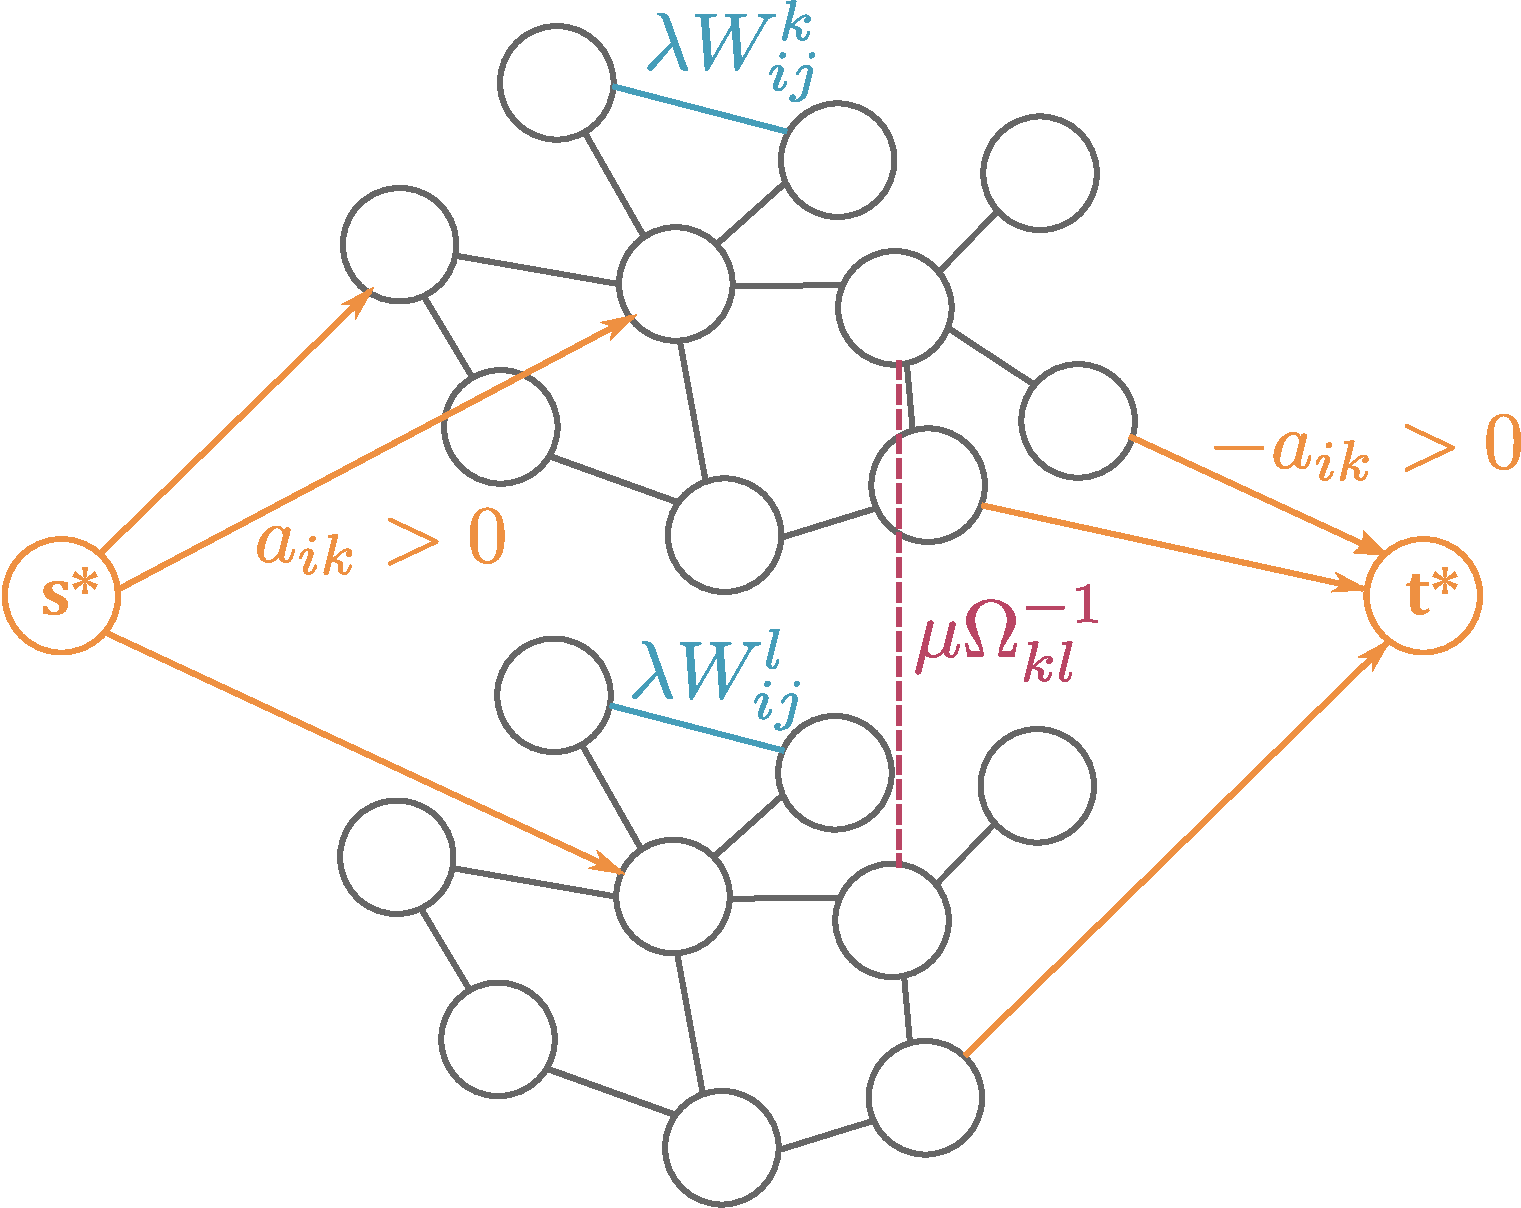
\includegraphics[width=0.7\textwidth]{figures/mincut_msfan}
  \caption{Finding the minimum cut of this super-network is equivalent to solving the multitask network-guided feature selection problem defined by Eq.~\ref{eq:msfan}.}
  \label{fig:mincut_msfan}
\end{figure}

\section{Range of hyperparameters}

To avoid trivial solutions (in which either all features or no features are selected), one must ensure that not all nodes are connected to the source (resp. sink). This implies that some values of $a_i^k$ are positive and others are negative.\\

By definition, $a_i^k = c_i^k - \mu \phi_k - \eta$. As
\[
\min_{i, k} c_i^k - \mu \max_k \phi_k - \eta \leq 
  a_i^k   \leq \max_{i, k} c_i^k - \mu \min_k \phi_k - \eta,
\]
this implies that $\min_{i, k} c_i^k - \mu \max_k \phi_k - \eta < 0$ and
$\max_{i, k} c_i^k - \mu \min_k \phi_k - \eta > 0$.\\

Hence, if $\mu$ is given, $\eta$ must be chosen smaller than 
$\max_{i, k} c_i^k - \mu \min_k \phi_k$.\\

Because we want $\eta$ to be strictly positive (to enforce sparsity), this in turn implies that\\ $\max_{i, k} c_i^k - \mu \min_k \phi_k > 0$. Hence our first condition:
\[ \mu < \frac{\max_{i, k} c_i^k}{\min_k \phi_k}.\]


We hence set $\mu_{\max} := \frac{\max_{i, k} c_i^k}{\min_k \phi_k}$.\\

In our experiments, we use $\mu \in \left\{ \frac{\mu_{\max}}{10 \times  2^t} \right \}_{t = 0, \dots, (T-1)}$.\\

$\mu$ being set, we can compute 
$\eta_{\max} := \max_{i, k} c_i^k - \mu \min_k \phi_k$ and use $\eta \in 
\left \{ \frac{\eta_{\max}}{10 \times 2^t} \right \}_{t = 0, \dots, (T-1)}$.\\

In order to make use of both the relevance scores and the network information, 
the values of $\lambda W_{ij}^k$ must be of similar magnitude to that of $|a_i^k|$. 
We take this to mean that $\lambda W_{ij}^k$ should take values spread around the median value of $|a_i^k|$,
between its largest and its smallest values.\\

Denoting by $W_{\min}$ the smallest non-zero value of $W$ : 
$W_{\min} := \min_{i, j, k} \{ W_{ij}^k | W_{ij}^k \neq 0\}$,
we propose to consider 
\[
\lambda_{\max} := \frac{\max_{i,k} |a_i^k|}{W_{\min}}, 
\lambda_{\min} := \frac{\min_{i,k} |a_i^k|}{\max_{i,j,k}W_{ij}^k} \mbox{ and }
\lambda_{m} := \frac{\mbox{median}_{i, k} |a_i^k|}{\max_{i,j,k}W_{ij}^k}.
\]

 We then use $\lambda \in \left \{ 10^ {\log_{10}(\lambda_{m}) - \frac{t}{(T+1)/2} 
 \left (\log_{10}(\lambda_{m}) - \log_{10}(\lambda_{\min}) \right)} \right \}_{t = 1, \dots, (T+1)/2}$ and

$\lambda \in \left \{ 10^ {\log_{10}(\lambda_{m}) + \frac{t}{T/2} 
\left (\log_{10}(\lambda_{\max}) - \log_{10}(\lambda_{m}) \right)} \right \}_{t = 0, \dots, T/2}$.



\paragraph{Remark.} In our experiments, we use a random sample of $50\%$ of the values of $c_i^k$ to set the ranges of values for the hyperparameters $\mu$, $\eta$ and $\lambda$ before starting.


\end{document}
